% Copyright 2004 by Till Tantau <tantau@users.sourceforge.net>.
%
% In principle, this file can be redistributed and/or modified under
% the terms of the GNU Public License, version 2.
%
% However, this file is supposed to be a template to be modified
% for your own needs. For this reason, if you use this file as a
% template and not specifically distribute it as part of a another
% package/program, I grant the extra permission to freely copy and
% modify this file as you see fit and even to delete this copyright
% notice. 

\documentclass{beamer}

% my preamble
\usepackage{amsmath,amssymb,graphicx}


% There are many different themes available for Beamer. A comprehensive
% list with examples is given here:
% http://deic.uab.es/~iblanes/beamer_gallery/index_by_theme.html
% You can uncomment the themes below if you would like to use a different
% one:
%\usetheme{AnnArbor}
%\usetheme{Antibes}
%\usetheme{Bergen}
%\usetheme{Berkeley}
%\usetheme{Berlin}
%\usetheme{Boadilla}
%\usetheme{boxes}
%\usetheme{CambridgeUS}
%\usetheme{Copenhagen}
%\usetheme{Darmstadt}
%\usetheme{default}
%\usetheme{Frankfurt}
%\usetheme{Goettingen}
%\usetheme{Hannover}
%\usetheme{Ilmenau}
%\usetheme{JuanLesPins}
%\usetheme{Luebeck}
\usetheme{Madrid}
%\usetheme{Malmoe}
%\usetheme{Marburg}
%\usetheme{Montpellier}
%\usetheme{PaloAlto}
%\usetheme{Pittsburgh}
%\usetheme{Rochester}
%\usetheme{Singapore}
%\usetheme{Szeged}
%\usetheme{Warsaw}

\title{PCM Clustering based on Noise Level}

% % A subtitle is optional and this may be deleted
% \subtitle{Optional Subtitle}

\author{Peixin~Hou\inst{1} \and Jiguang~Yue\inst{1} \and Hao~Deng\inst{2} \and Shuguang~Liu\inst{3}}
% - Give the names in the same order as the appear in the paper.
% - Use the \inst{?} command only if the authors have different
%   affiliation.

\institute[Universities] % (optional, but mostly needed)
{
  \inst{1}%
  Department of Control Science and Engineering, Tongji University
  \and
  \inst{2}%
  School of Physics and Electronics, Henan University
  \and
  \inst{3}%
  Department of Hydraulic Engineering, Tongji University
  }
% - Use the \inst command only if there are several affiliations.
% - Keep it simple, no one is interested in your street address.

\date{FUZZ-IEEE, 2017}
% - Either use conference name or its abbreviation.
% - Not really informative to the audience, more for people (including
%   yourself) who are reading the slides online

\subject{Fuzzy Clustering}
% This is only inserted into the PDF information catalog. Can be left
% out. 

% If you have a file called "university-logo-filename.xxx", where xxx
% is a graphic format that can be processed by latex or pdflatex,
% resp., then you can add a logo as follows:

\pgfdeclareimage[height=0.5cm]{university-logo}{tongji-university-logo}
%\pgfdeclareimage[height=0.5cm]{university-logo}{Tongji_Uni_logo}
\logo{\pgfuseimage{university-logo}}

% Delete this, if you do not want the table of contents to pop up at
% the beginning of each subsection:
\AtBeginSubsection[]
{
  \begin{frame}<beamer>{Outline}
    \tableofcontents[currentsection,currentsubsection]
  \end{frame}
}

% Let's get started
\begin{document}

\begin{frame}
  \titlepage
\end{frame}

\begin{frame}{Outline}
  \tableofcontents
  % You might wish to add the option [pausesections]
\end{frame}

% Section and subsections will appear in the presentation overview and
% table of contents.

\section{Introduction}

\begin{frame}
  \frametitle{Introduction}
  How much information we should provide for the clustering algorithm
  in order to discover the natural (physical) clusters?
  \begin{itemize}
  \item information of the cluster number \pause
  \item information of the property (e.g., density or closeness) of
    clusters.
  \end{itemize}
\end{frame}

\begin{frame}
  \frametitle{Our Main Contributions}
  \begin{itemize}
  \item The proposed NPCM have two parameters, where $m_{ini}$ is a
    possibly over-specified cluster number, and $\alpha$ characterizes
    the closeness of clusters in the clustering result.
  \item Both parameters are not required to be exactly specified.
  \end{itemize}
  
\end{frame}


\section{The PCM Based Algorithms}


\begin{frame}{The PCM Algorithm}
  The objective of possibilistic c-means (PCM)
  \cite{krishnapuram_possibilistic_1993} is to minimize the following
  cost:
  \begin{equation}
    J(\mathbf{\Theta},\mathbf{U})=\sum_{j=1}^{c}J_j=\sum_{j=1}^{c}\left[\sum_{i=1}^{N}u_{ij}d_{ij}^2+\gamma_j \sum_{i=1}^{N}f(u_{ij})\right]
  \end{equation}
  where $f(\cdot)$ can be chosen as:
  \begin{equation}
    f(u_{ij})=u_{ij}\log u_{ij}-u_{ij}.
  \end{equation}
\end{frame}

\begin{frame}
  \frametitle{The PCM Algorithm}
  Minimizing $J(\mathbf{\Theta},\mathbf{U})$ with respect to $u_{ij}$
  and $\boldsymbol{\theta}_j$ leads to the following two update
  equations:
  \begin{align}
    u_{ij}&=\exp\left(-\frac{d^2_{ij}}{\gamma_j}\right) \label{pcm_u_update}  \\
    \boldsymbol{\theta}_j&=\frac{\Sigma_{i=1}^Nu_{ij}\mathbf{x}_i}{\Sigma_{i=1}^Nu_{ij}} \label{pcm_theta_update}    
  \end{align}
\end{frame}

\begin{frame}
  \begin{columns}[t]
    \column{.45\textwidth}
    
    \begin{block}{Drawback of PCM}
      \begin{itemize}
      \item $\gamma_j$ is fixed after initialization, so its
        performance relies heavily on good initial partitions and
        parameters \cite{nasraoui_improved_1996}.
      \item<2> The $c$ dense regions found may be coincident
        \cite{barni_comments_1996}.
      \end{itemize}
    \end{block}

    \column{.5\textwidth}
    \begin{block}{Improvement of Adaptive PCM
        \cite{xenaki_novel_2016}}
      \begin{itemize}
      \item Adapt $\gamma_j$ at each iteration.  \vskip2cm
      \item<2> The clusters with $\gamma_j=0$ are eliminated.
      \end{itemize}
    \end{block}
  \end{columns}
\end{frame}

\begin{frame}
  \frametitle{The APCM Algorithm}
  The price of Adaptive PCM (APCM): introduce another parameter
  $\alpha$ to manually control the process of adaptive $\alpha_j$.
  \begin{equation}
    \label{corrected_eta}
    \gamma_j=\frac{\hat{\eta}}{\alpha}\eta_j
  \end{equation}
  $\hat{\eta}$ is initialized in the first iteration. \\
  Let $A_j=\{\mathbf{x}_i|u_{ij}=\max_r u_{ir}\}$. $\eta_j$ is updated
  at each iteration as:
  \begin{equation}
    \label{apcm_eta_update}
    \eta_j=\frac{1}{n_j}\sum_{\mathbf{x}_i\in A_j}||\mathbf{x}_i-\boldsymbol{\mu}_j||
  \end{equation}
  where $n_j$ and $\boldsymbol{\mu}_j$ are the number of points in
  $A_j$ and the mean vector of points in $A_j$ respectively.
\end{frame}

\begin{frame}
  \frametitle{What APCM Acutually Does}
  Introduce parameter $\alpha$ to correct the estimated bandwidth
  $\eta_j$, so that the corrected bandwidth \eqref{corrected_eta}
  approximates the true one.
 
\end{frame}

\begin{frame}
  \frametitle{The UPCM Algorithm: an alternate Bandwidth Correction
    Method}
  In the UPCM paper \cite{hou_pcm_2016}, the bandwidth correction
  process is performed in a more fuzzy way by utilizing the
  conditional fuzzy set framework \cite{wang_new_2016}:
  \begin{equation}
    \label{upcm_u_update}
    \mu_{ij}=\exp\left(-\frac{d_{ij}^2}{\gamma_j}\right)
  \end{equation}
  where
  $\gamma_j=\left(0.5\eta_{j}+0.5\sqrt{\eta_{j}^{2}+4\sigma_vd_{ij}}\right)^2$
  and $\sigma_v$ controls the uncertainty of the estimated bandwidth.
\end{frame}


\begin{frame}
  \frametitle{The UPCM Algorithm: an alternate Bandwidth Correction
    Method}
  UPCM also introduces the concept of \emph{noise level} $\alpha$ of
  the data set in the update equation of prototypes:
  \begin{equation}
    \label{upcm_theta_update}
    \boldsymbol{\theta}_j=\frac{\Sigma_{i=1}^Nu_{ij}\mathbf{x}_i}{\Sigma_{i=1}^Nu_{ij}} \quad \text{for}\;u_{ij}\geq \alpha.
  \end{equation}
  By setting an appropriate $\alpha$, the influence of points in other
  clusters $\boldsymbol{\theta}_{i\neq j}$ on the
  $\boldsymbol{\theta}_j$ update is reduced.
\end{frame}

\section{An Impression of the Algorithms' Performence}




\begin{frame}
  \begin{center}
    Dataset 1 (upper) and Dataset 2 (lower) and their initializations\\
    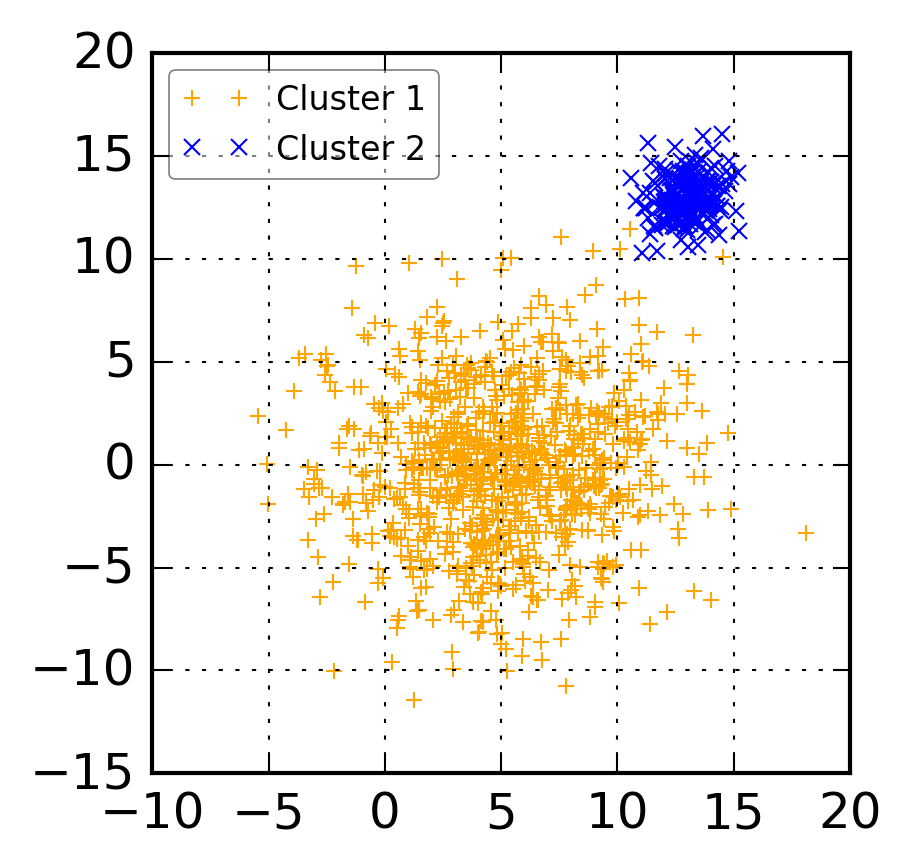
\includegraphics[height=4cm]{img/exmp_dif_variance_ori.png}
    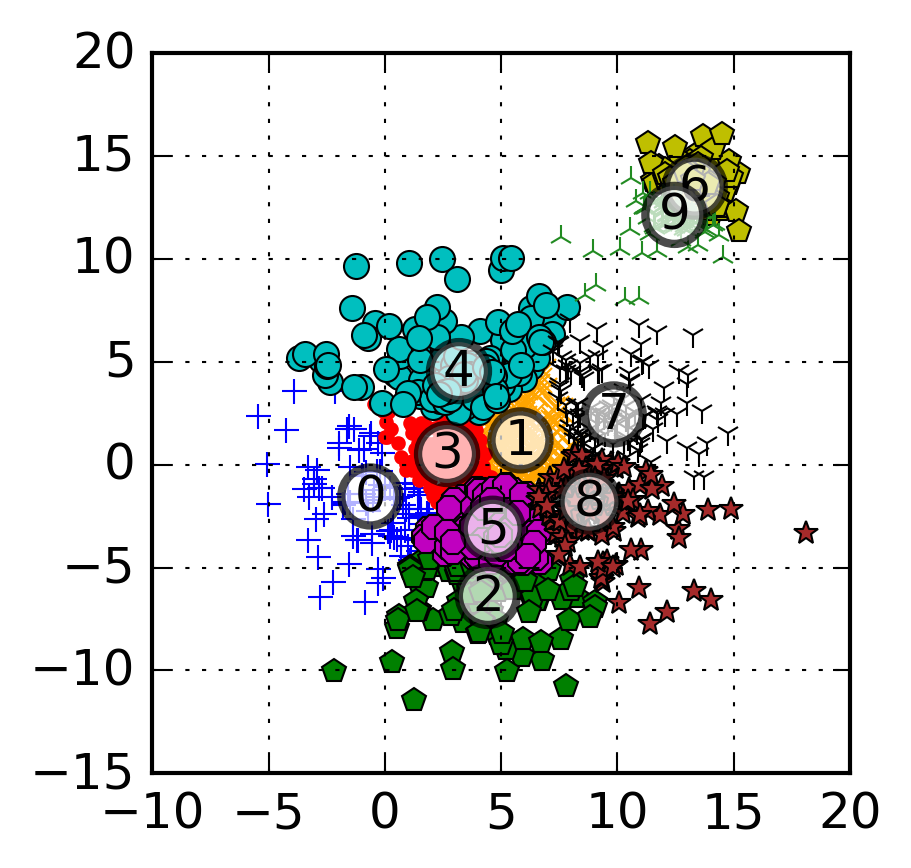
\includegraphics[height=4cm]{img/exmp_dif_variance_ini.png}
  \end{center}

  \begin{center}
    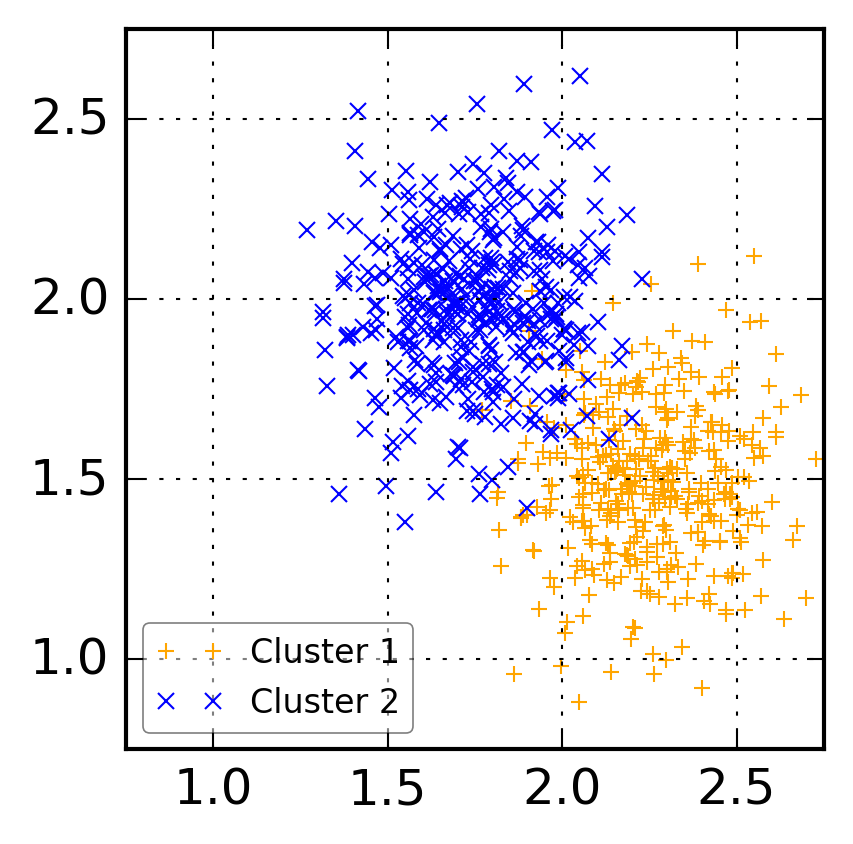
\includegraphics[height=4cm]{img/exmp_close_ori.png}
    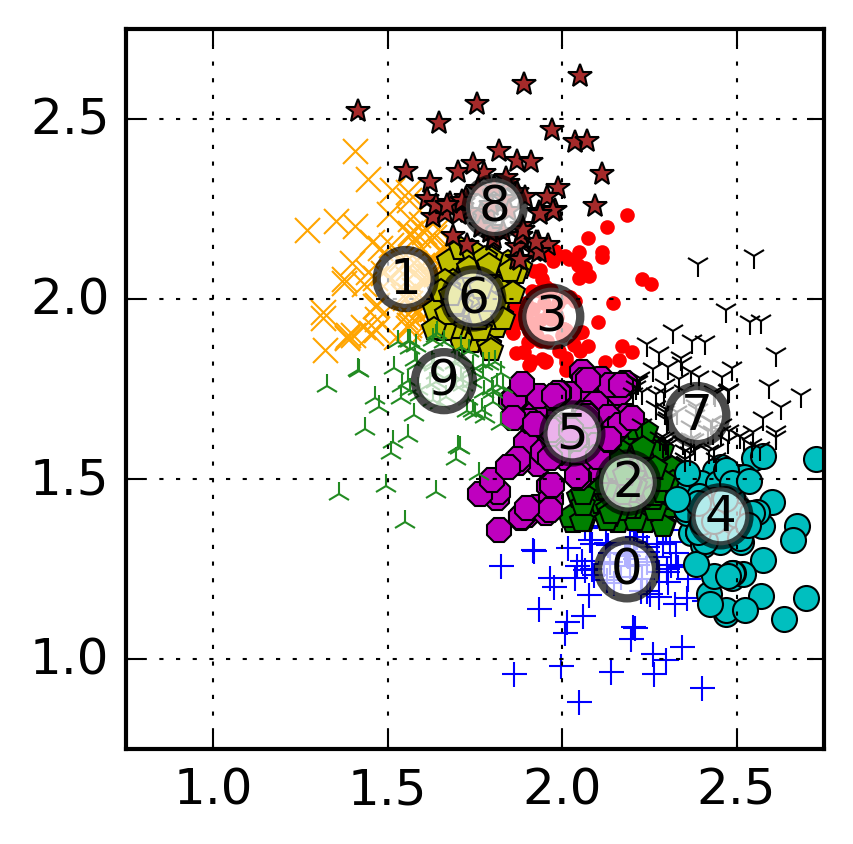
\includegraphics[height=4cm]{img/exmp_close_ini.png}
    \vskip1cm
  \end{center}
\end{frame}

\begin{frame}
  \frametitle{The Final Cluster Number of APCM}
  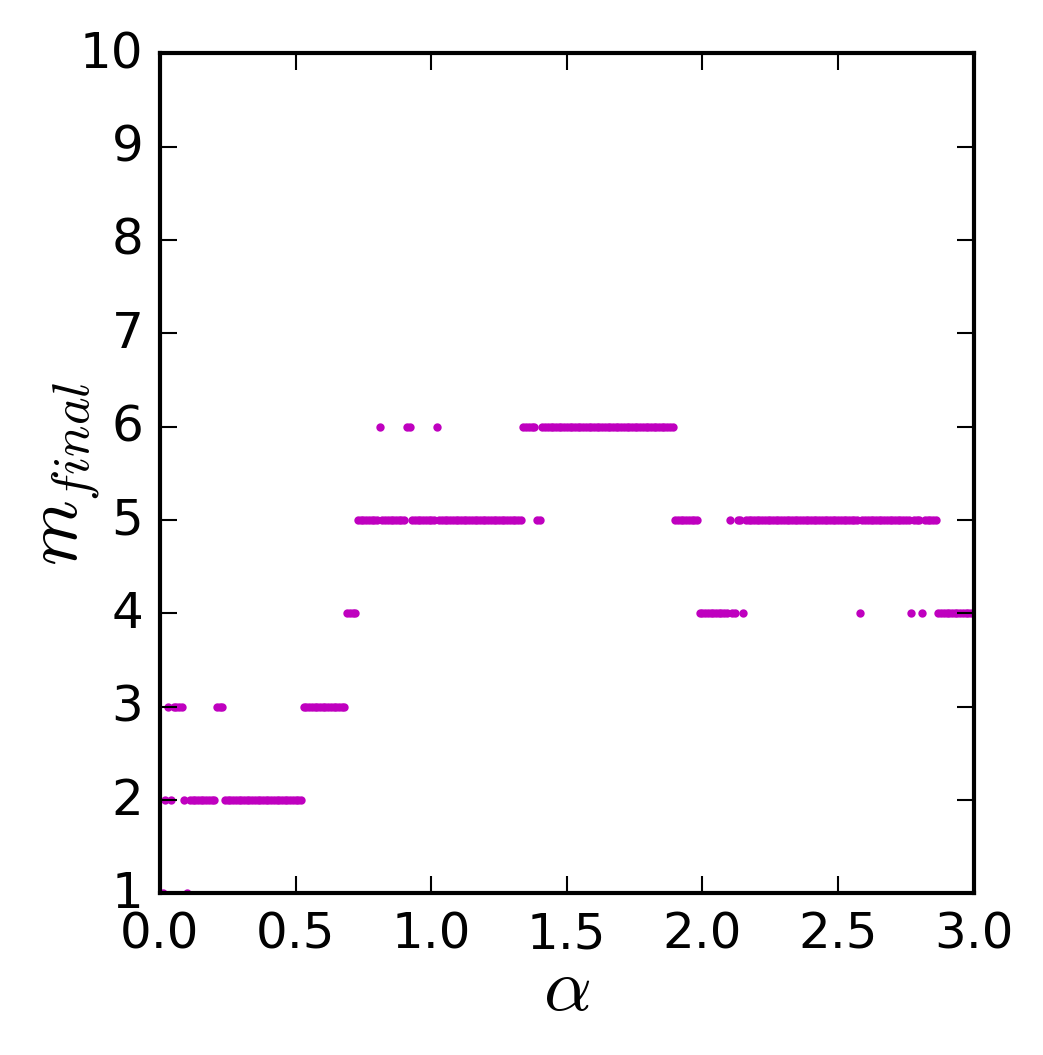
\includegraphics[width=0.5\columnwidth]{img/exmp_apcm_dif_var.png}
  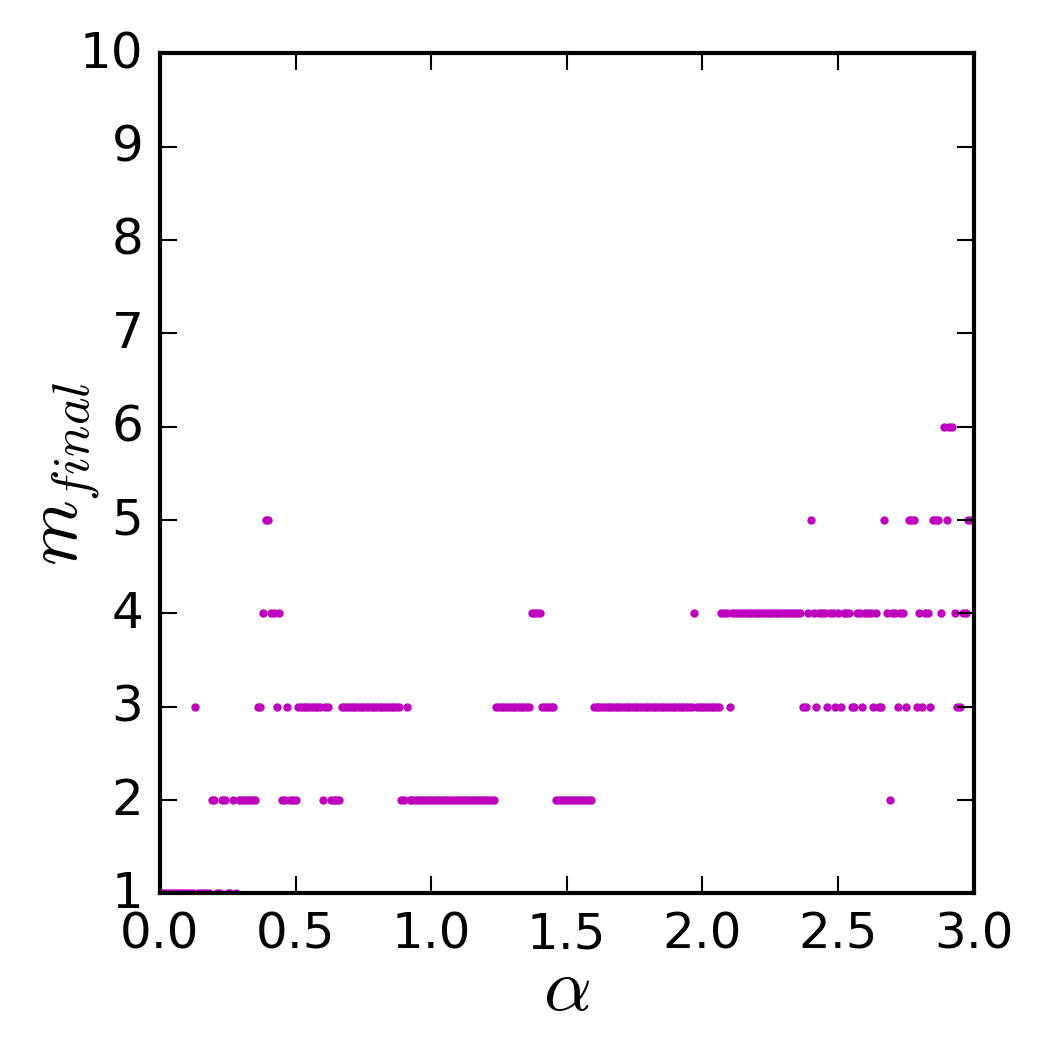
\includegraphics[width=0.5\columnwidth]{img/exmp_apcm_close.png} \\
  Result on Dataset 1 (left) and Dataset 2 (right)
\end{frame}


\begin{frame}
  \frametitle{The Final Cluster Number of UPCM}
  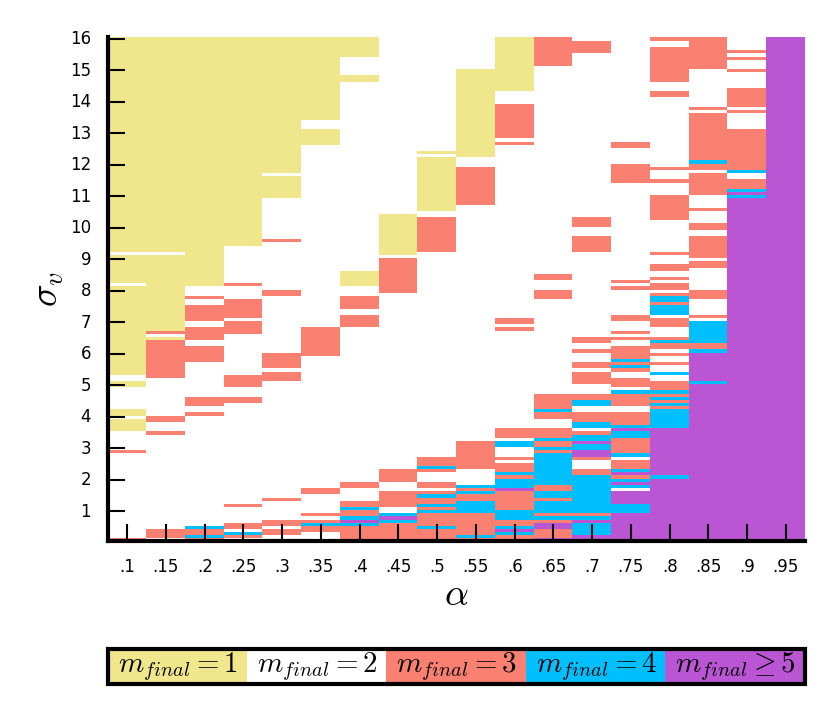
\includegraphics[width=0.5\textwidth]{img/exmp_dif_variance_scan.png}
  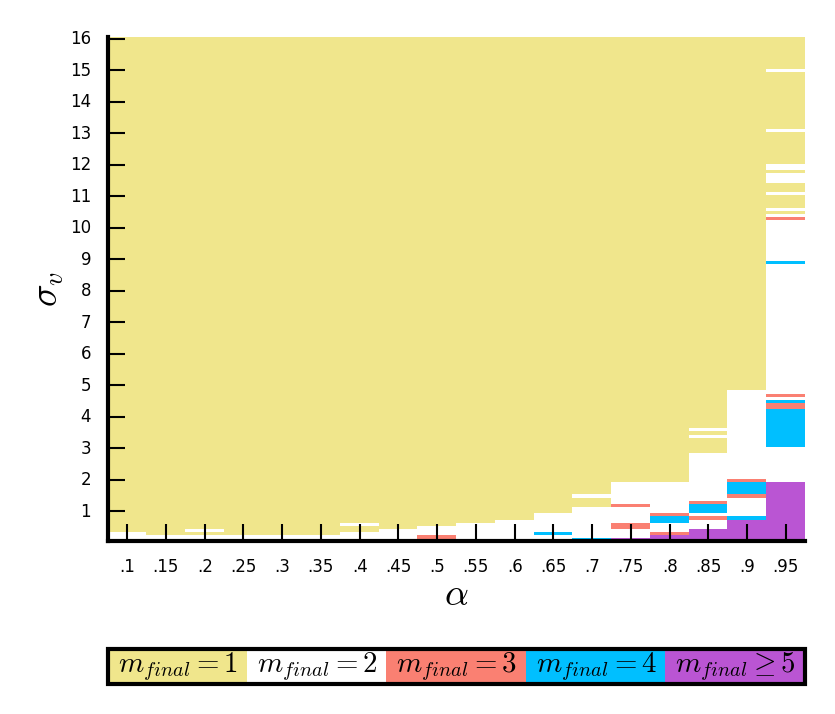
\includegraphics[width=0.5\textwidth]{img/exmp_close_scan.png}
  \\
  Result on Dataset 1 (left) and Dataset 2 (right)
\end{frame}

\begin{frame}
  \frametitle{The Final Cluster Number of NPCM}
  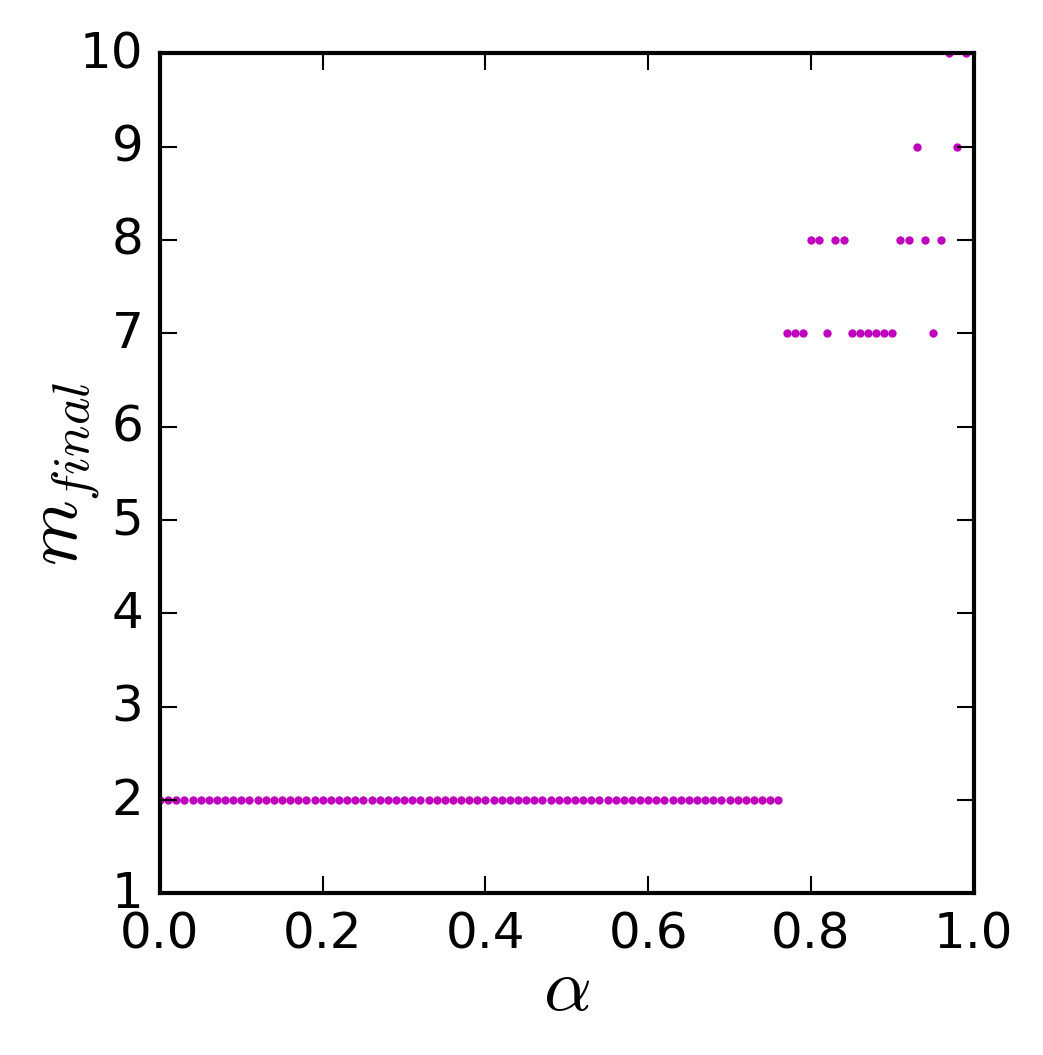
\includegraphics[width=0.5\columnwidth]{img/exmp_npcm_fcm_dif_variance.png}
  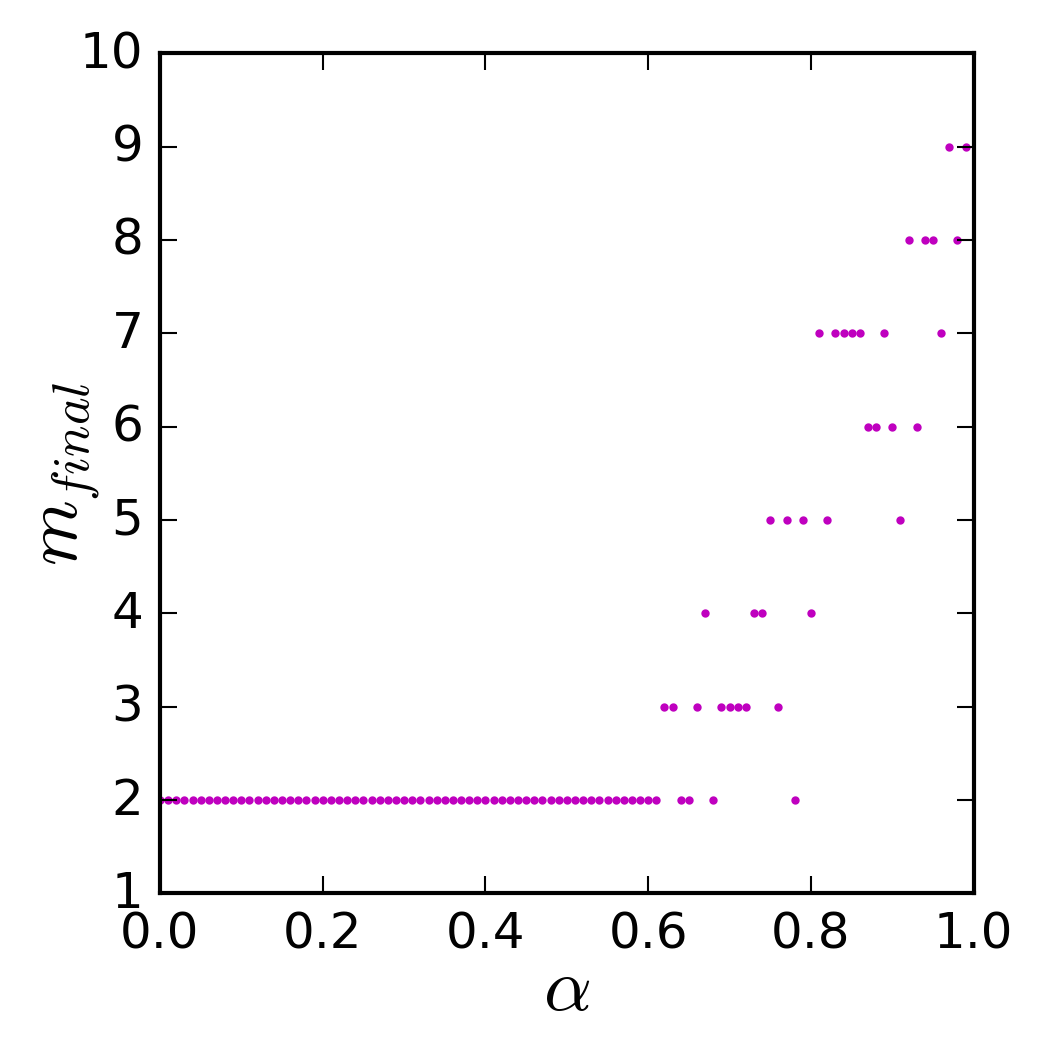
\includegraphics[width=0.5\columnwidth]{img/exmp_npcm_fcm_close.png}
  \\
  Result on Dataset 1 (left) and Dataset 2 (right)
\end{frame}

\section{Algorithm Development}


\begin{frame}
  \frametitle{Motivation of This Paper}
  \begin{itemize}
  \item {UPCM has two hyperparameters, i.e., $\alpha$ and
      $\sigma_v$. It's possible to eliminate parameter $\sigma_v$}
    \pause
  \item Both APCM and UPCM suffer from the problem of background noise
    clusters, i.e., the background noise clusters are highly possible
    to become very large.
  \end{itemize}
\end{frame}

\begin{frame}
  \frametitle{Algorithm Outline}
  \includegraphics[width=\columnwidth]{img/outline_algorithm_development.pdf}
\end{frame}


\begin{frame}
  \frametitle{The Background Noise Problem}
  \begin{center}
    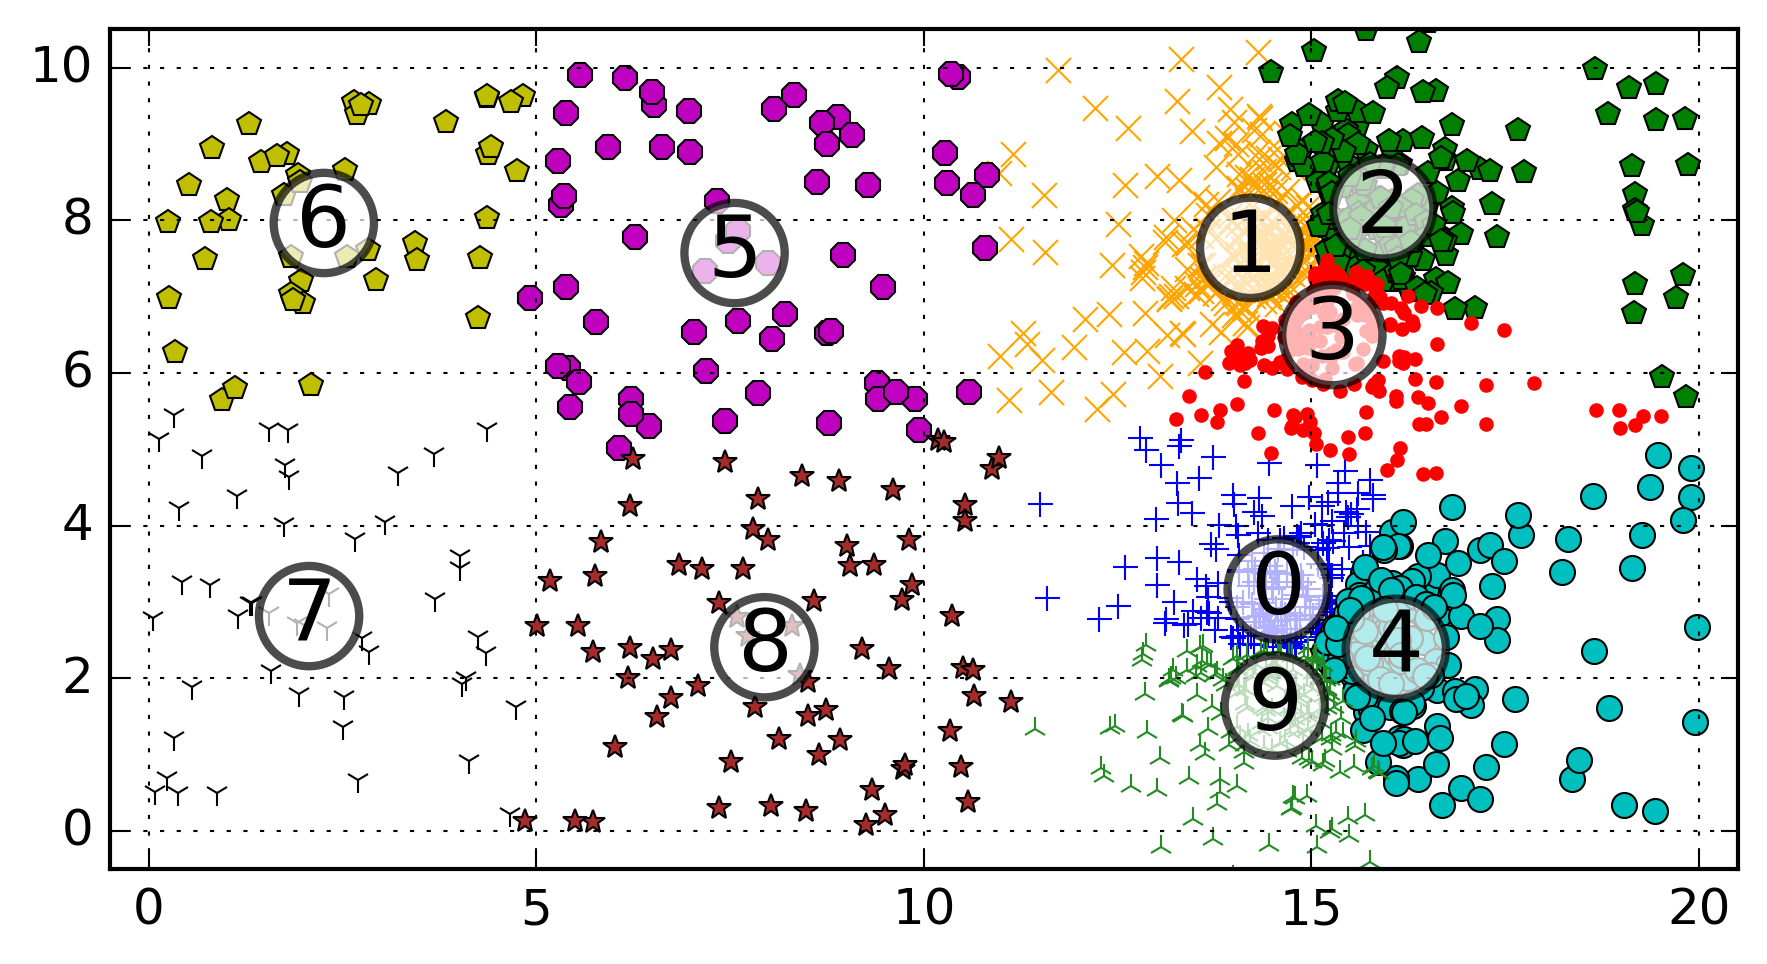
\includegraphics[height=4cm]{img/noise_cluster_problem_ini.png} \\
    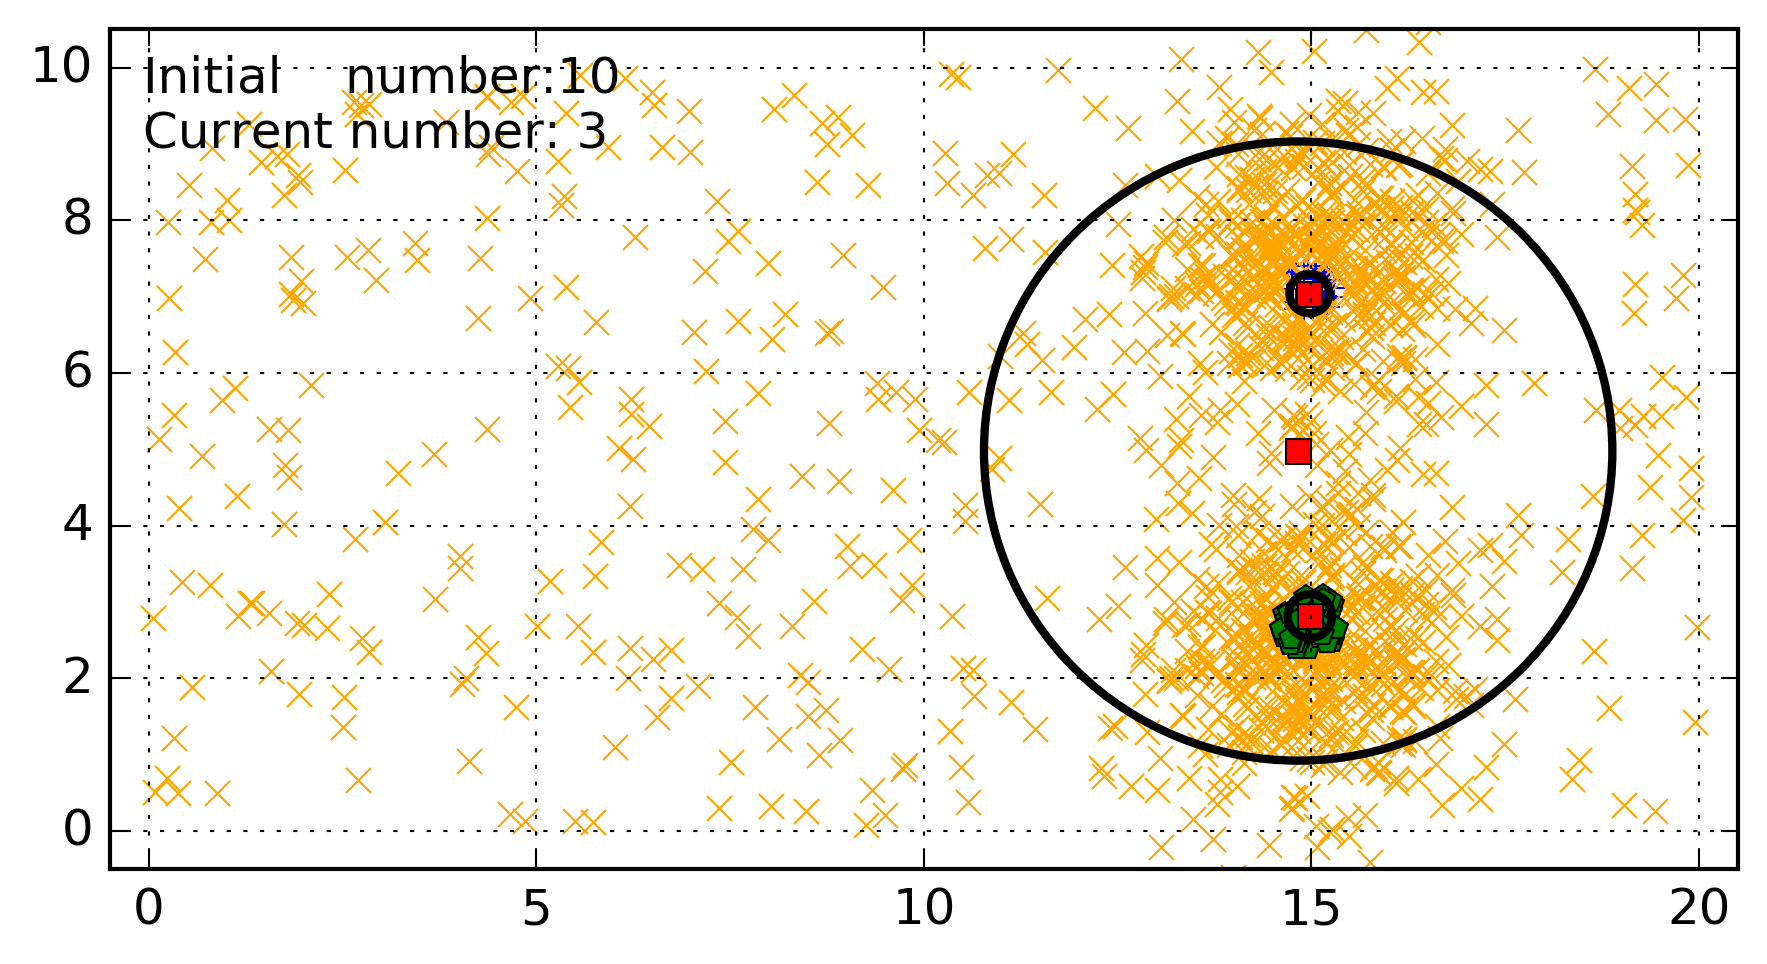
\includegraphics[height=4cm]{img/noise_cluster_problem_last_frame.png}
  \end{center}
\end{frame}

\begin{frame}
  \frametitle{Eliminate Noise Clusters}
  Define the density of a cluster as:
  \begin{equation}
    \label{npcm_density}
    \rho_j=\frac{n_j}{\eta_j^d}
  \end{equation}
  where $d$ is the dimension of $\mathbf{x}_i$. Let
  $\rho_0=\max_j\rho_j$. Then the cluster $C_j$ is considered as a
  noise cluster and is eliminated if $\rho_j<0.1\rho_0$.
\end{frame}


\begin{frame}
  \frametitle{Modeling the Relation Between $\alpha$ and $\sigma_v$}
  We can calculate the distance $d_{j\alpha}$ beyond which a point
  can't be used to contribute to the adaption of cluster $C_j$ by
  letting
  \begin{equation}
    \exp\left(-\frac{(d_{j\alpha})^2}{\gamma_j}\right)=\alpha,
  \end{equation}
  which leads to
  \begin{equation}
    \label{npcm_d_alpha}
    d_{j\alpha}=\sqrt{-\ln\alpha}\left(\eta_j+\sqrt{-\ln\alpha}\sigma_v\right).
  \end{equation}

  When there is no uncertainty in the estimated bandwidth, we get
  $d_{j\alpha}^0=\sqrt{-\ln\alpha}\eta_j$.
\end{frame}

\begin{frame}
  We fix the effect of $\sigma_v$ as the correction of $d_{j\alpha}^0$
  by considering the uncertainty of the estimated bandwidth
  \begin{equation}
    \frac{d_{j\alpha}-d_{j\alpha}^0}{d_{j\alpha}^0}=\frac{\sqrt{-\ln\alpha}\sigma_v}{\eta_j}=\beta,
  \end{equation}
  which leads to
  \begin{equation}
    \label{npcm_sig_alpha_relation}
    \sigma_v=\beta\frac{\eta_j}{\sqrt{-\ln\alpha}}.
  \end{equation}
  where $\beta$ characterizes the correction degree.  In this paper,
  we choose $\beta=0.2$.
\end{frame}

\begin{frame}
  The update of the membership function is then modified according to
  \eqref{upcm_u_update} and \eqref{npcm_sig_alpha_relation} as:
  \begin{equation}
    \label{npcm_u_update}
    \mu_{ij}=\exp\left(-\frac{d_{ij}^2}{\gamma_j}\right)
  \end{equation}
  where
  $\gamma_j=\left(0.5\eta_{j}+0.5\sqrt{\eta_{j}^{2}+0.8d_{ij}\eta_j/\sqrt{-\ln\alpha}}\right)^2$
  and $d_{ij}=||\mathbf{x}_i-\boldsymbol{\theta}_j||$.
\end{frame}

\section{Experiments}

\subsection{Experiment 1}


\begin{frame}
  \frametitle{Experiment 1}
  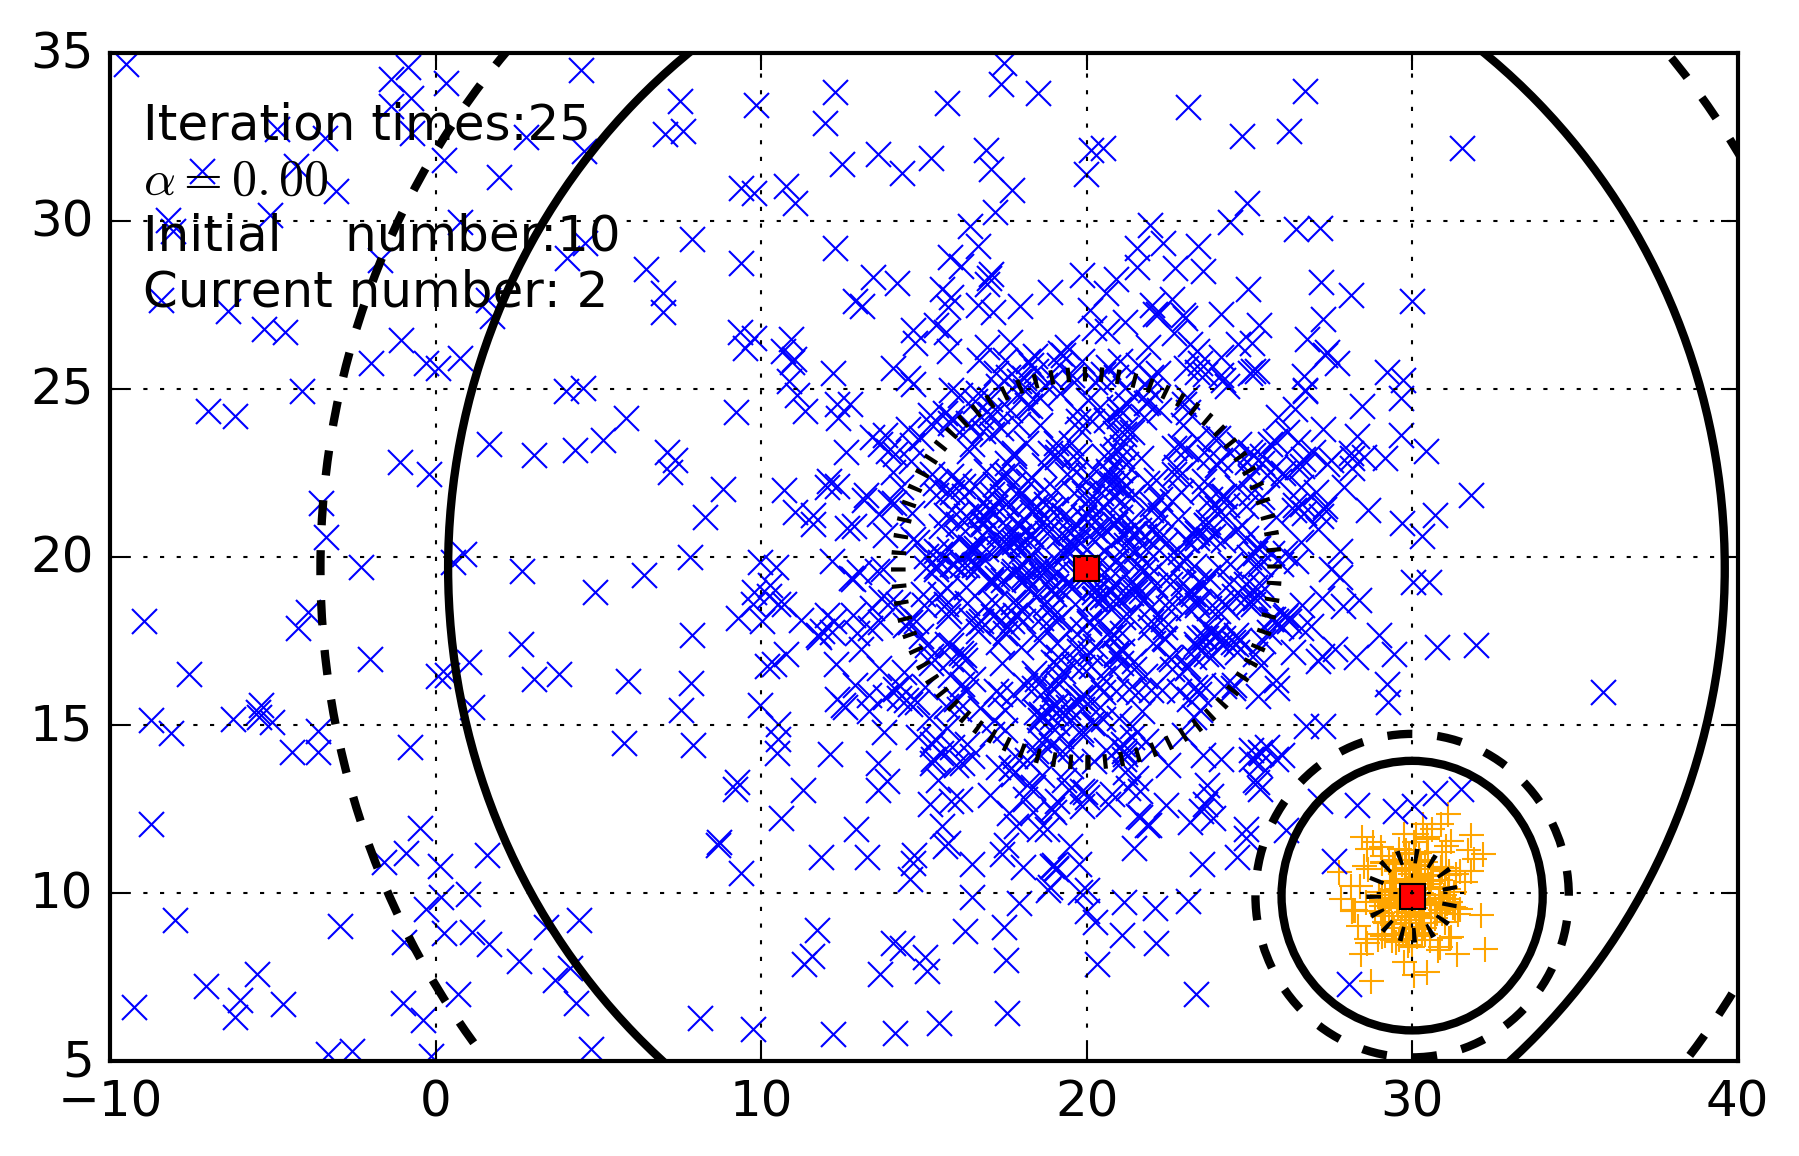
\includegraphics[height=7cm]{img/small_cluster_structure_preserve_last_frame_n_10_alpha_0_0.png}
\end{frame}

\begin{frame}
  \frametitle{Experiment 1}
  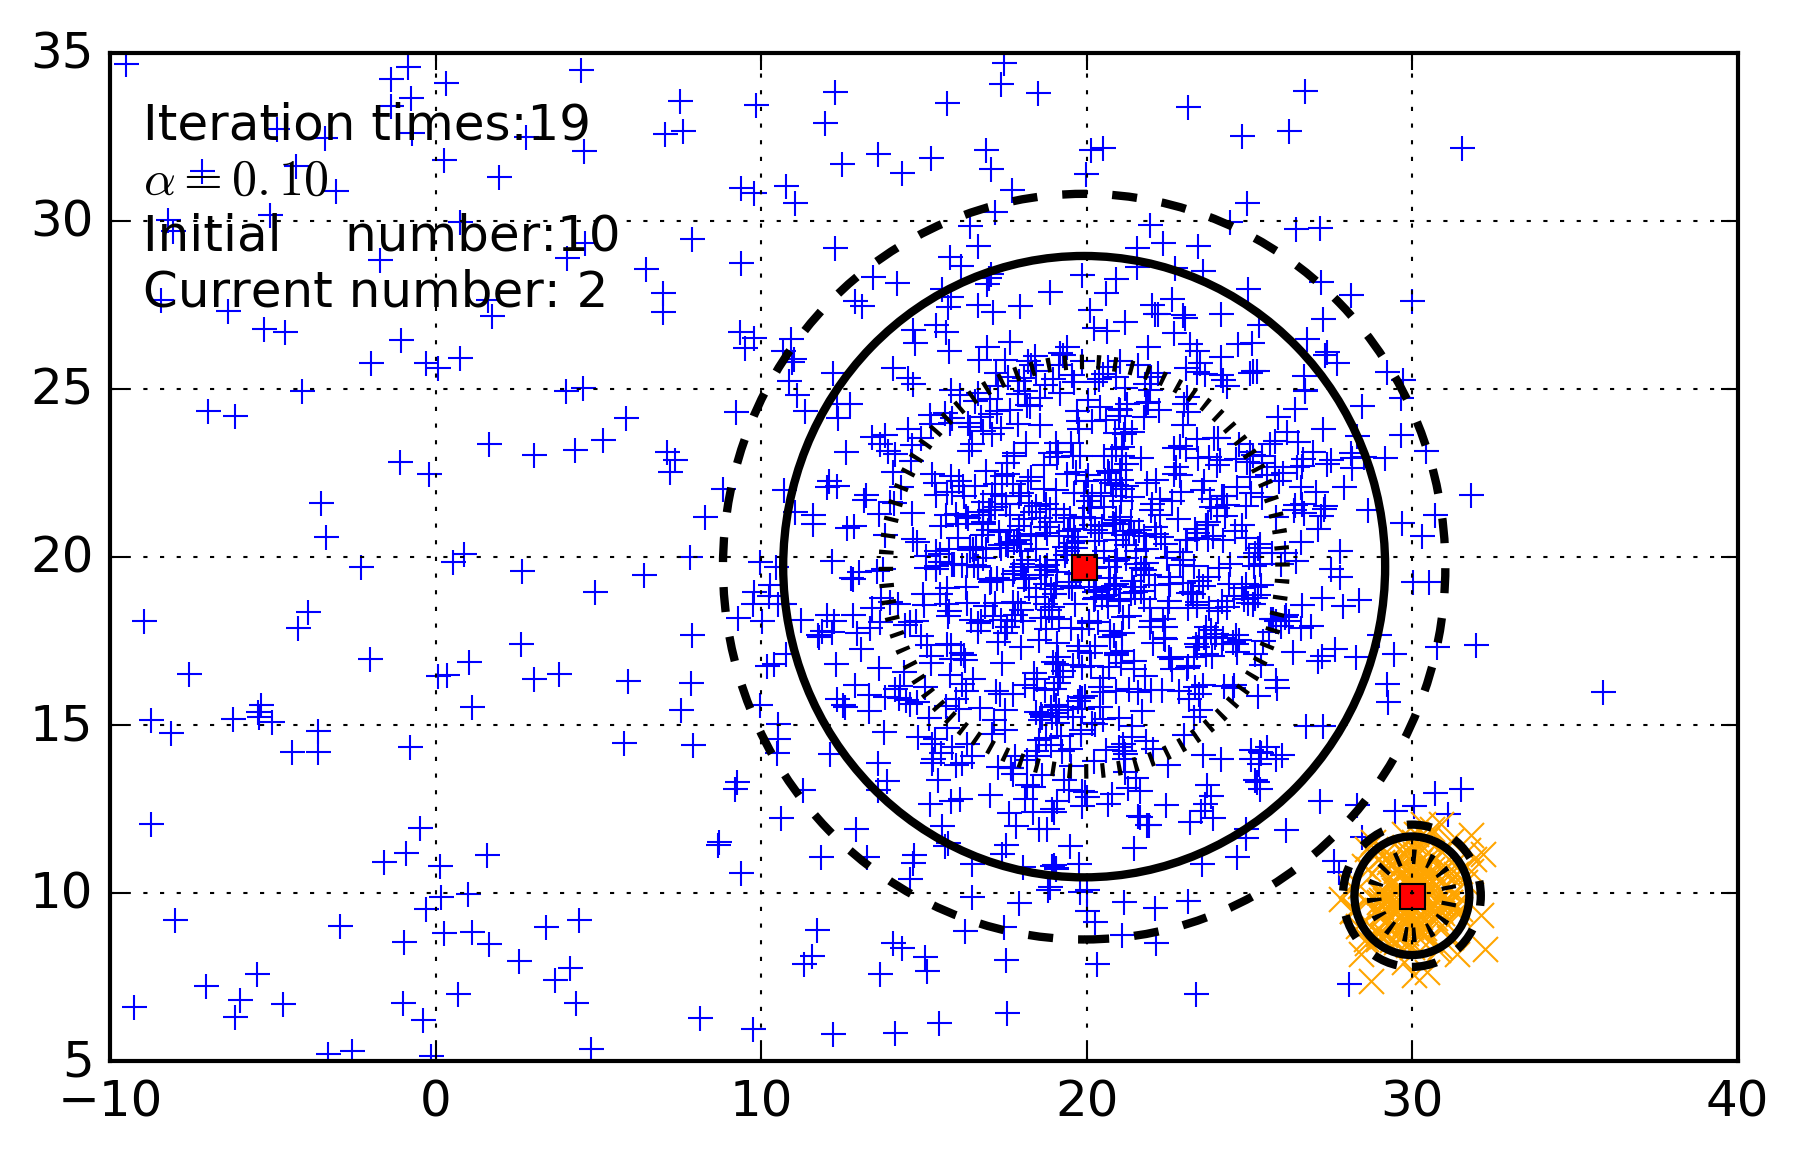
\includegraphics[height=7cm]{img/small_cluster_structure_preserve_last_frame_n_10_alpha_0_1.png}
\end{frame}

\begin{frame}
  \frametitle{Experiment 1}
  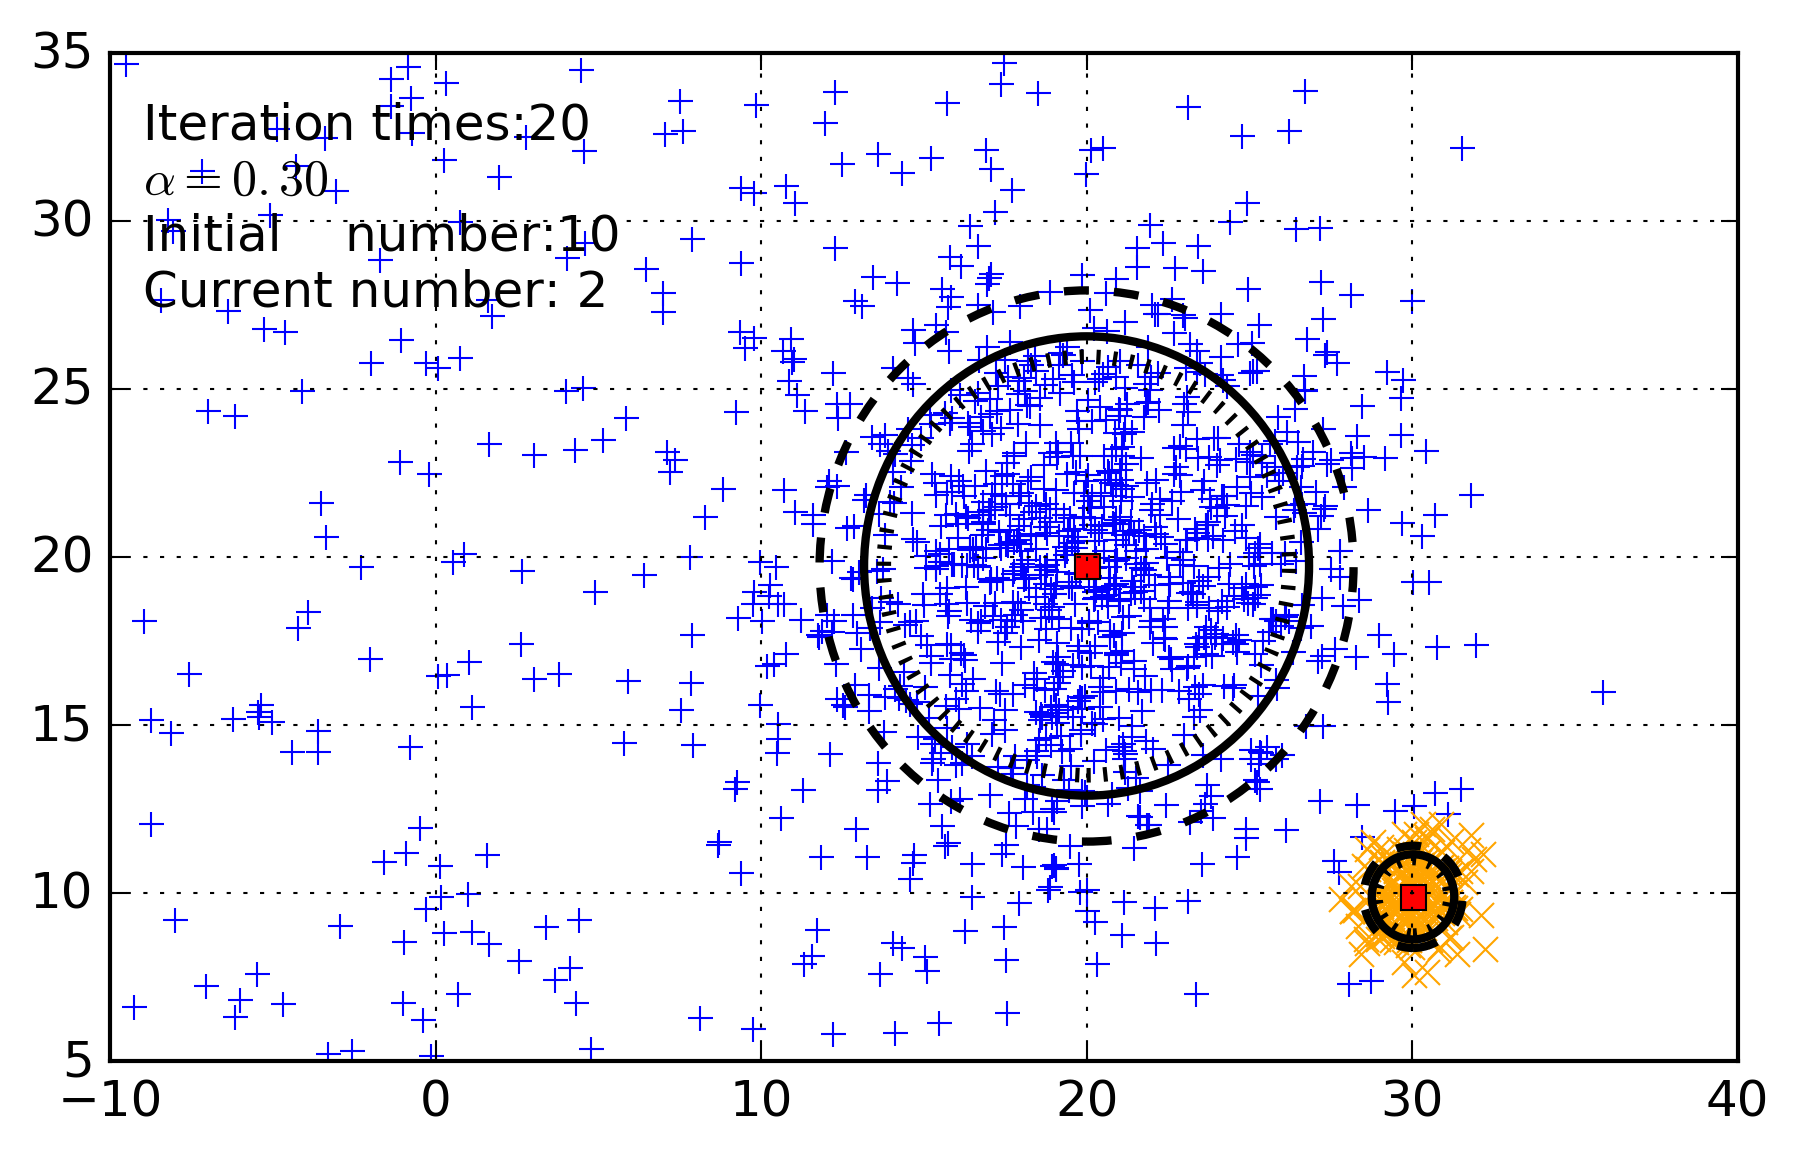
\includegraphics[height=7cm]{img/small_cluster_structure_preserve_last_frame_n_10_alpha_0_3.png}
\end{frame}

\begin{frame}
  \frametitle{Experiment 1}
  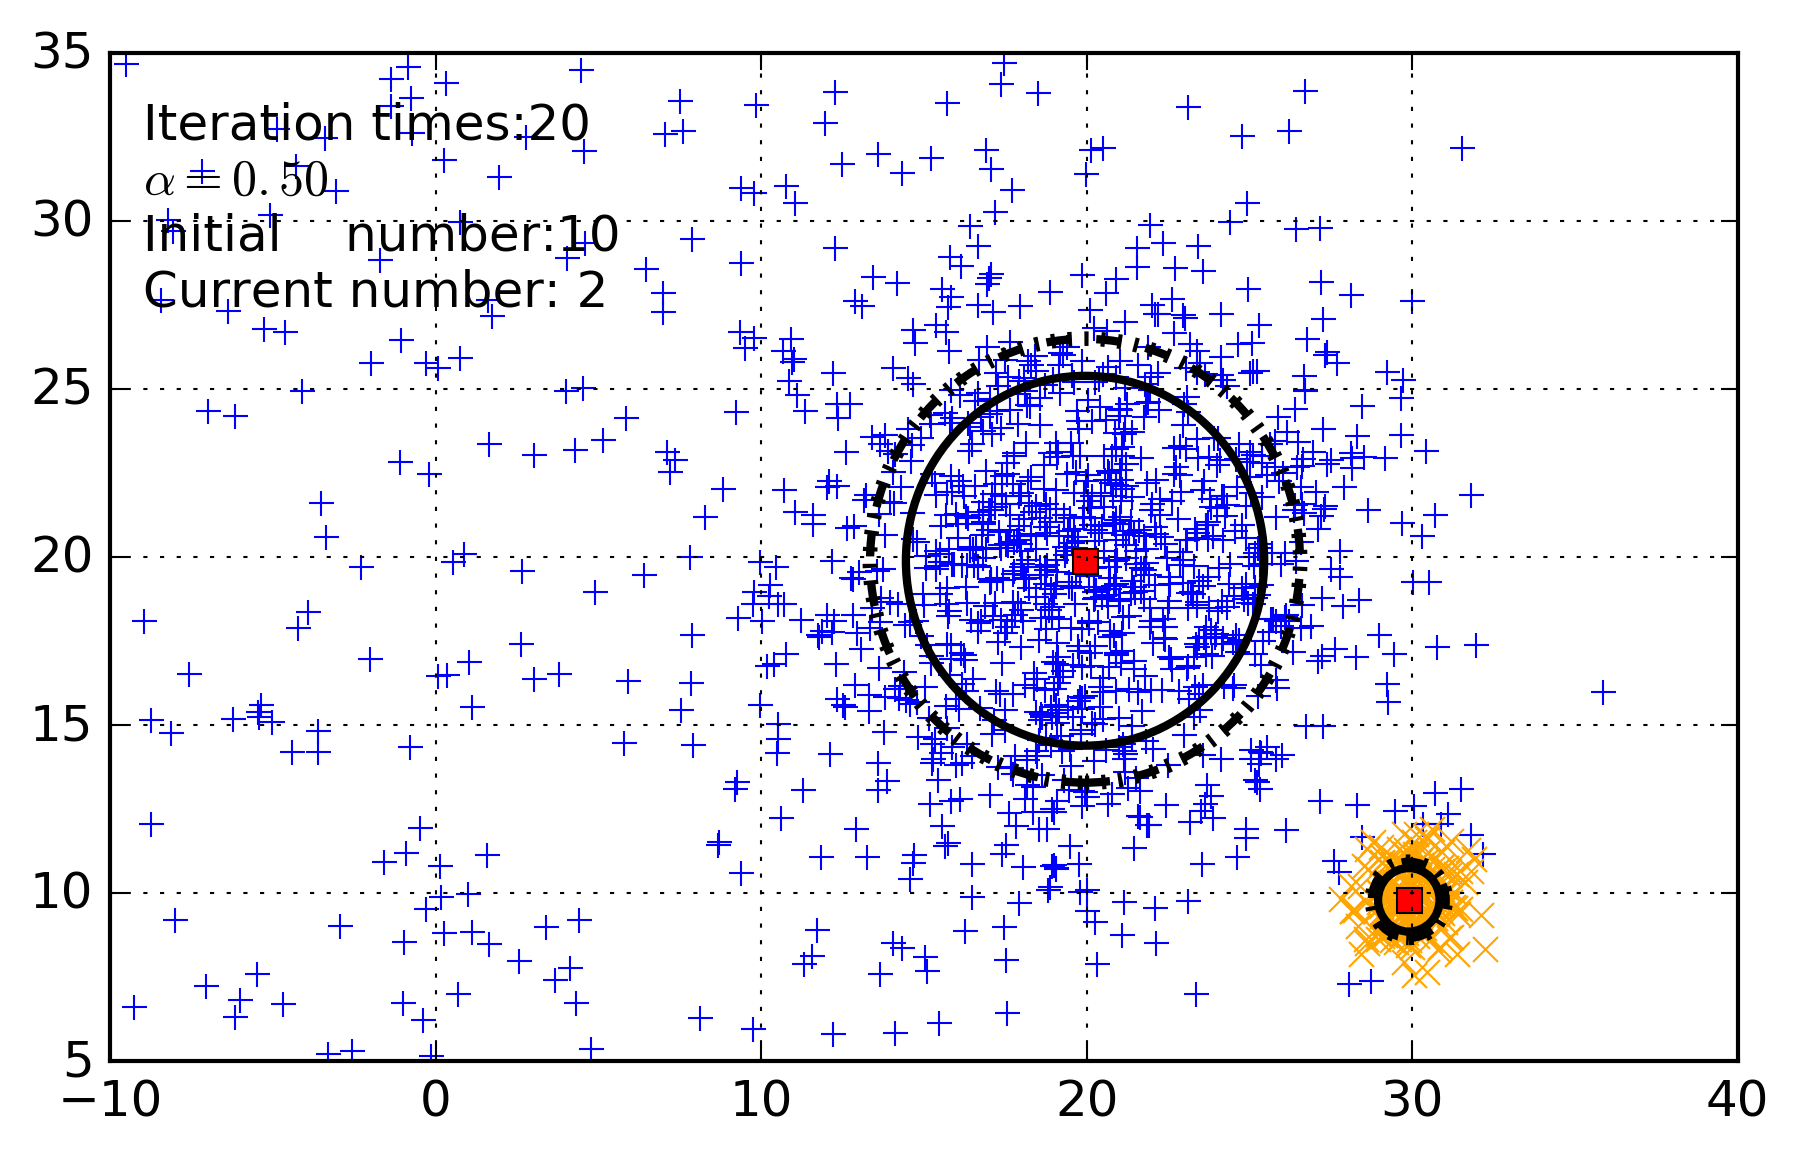
\includegraphics[height=7cm]{img/small_cluster_structure_preserve_last_frame_n_10_alpha_0_5.png}
\end{frame}

\subsection{Experiment 2}


\begin{frame}
  \frametitle{Experiment 2}
  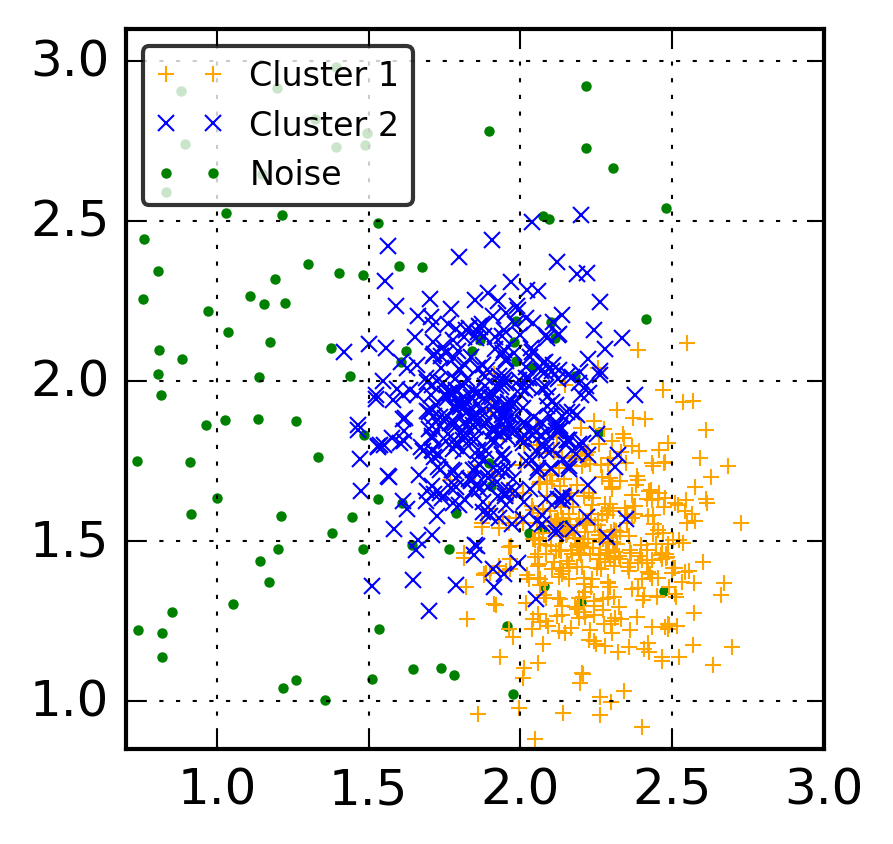
\includegraphics[width=0.33\textwidth]{img/example_close_cluster_ori.png}
  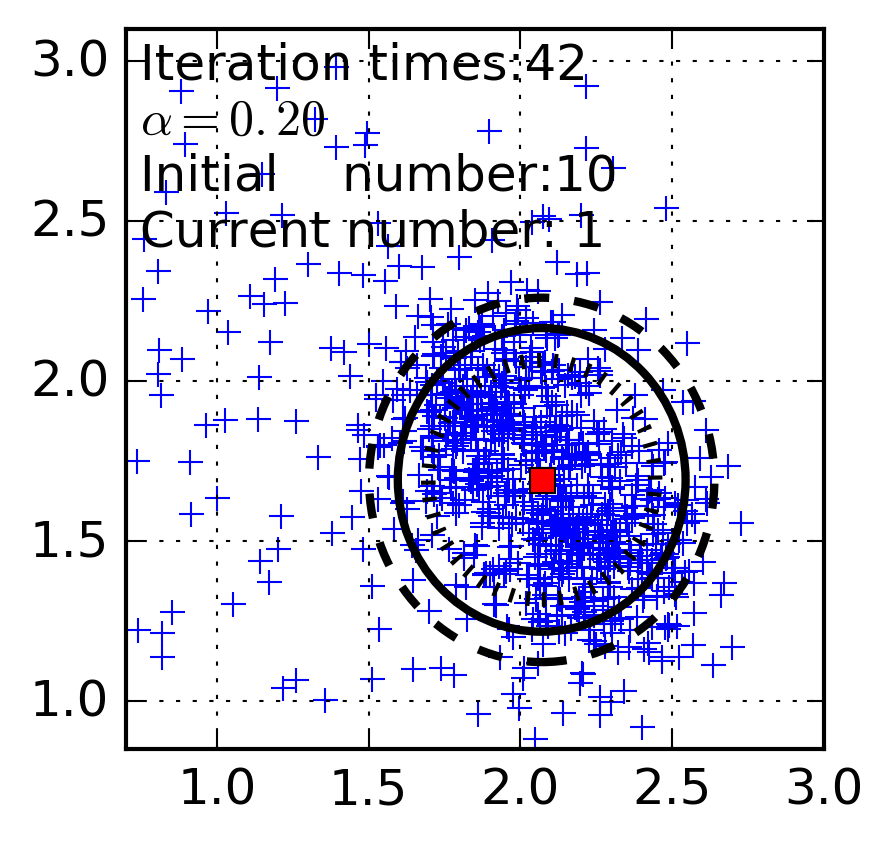
\includegraphics[width=0.33\textwidth]{img/example_close_cluster_last_frame_n_10_alpha_0_2.png}
  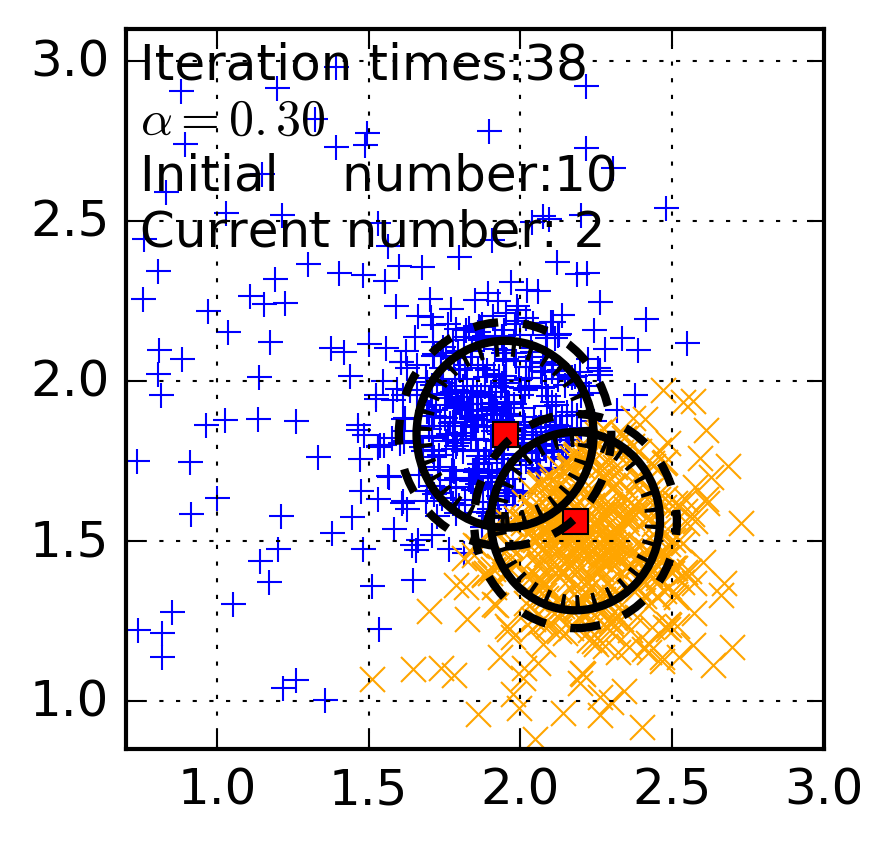
\includegraphics[width=0.33\textwidth]{img/example_close_cluster_last_frame_n_10_alpha_0_3.png}
  \\
  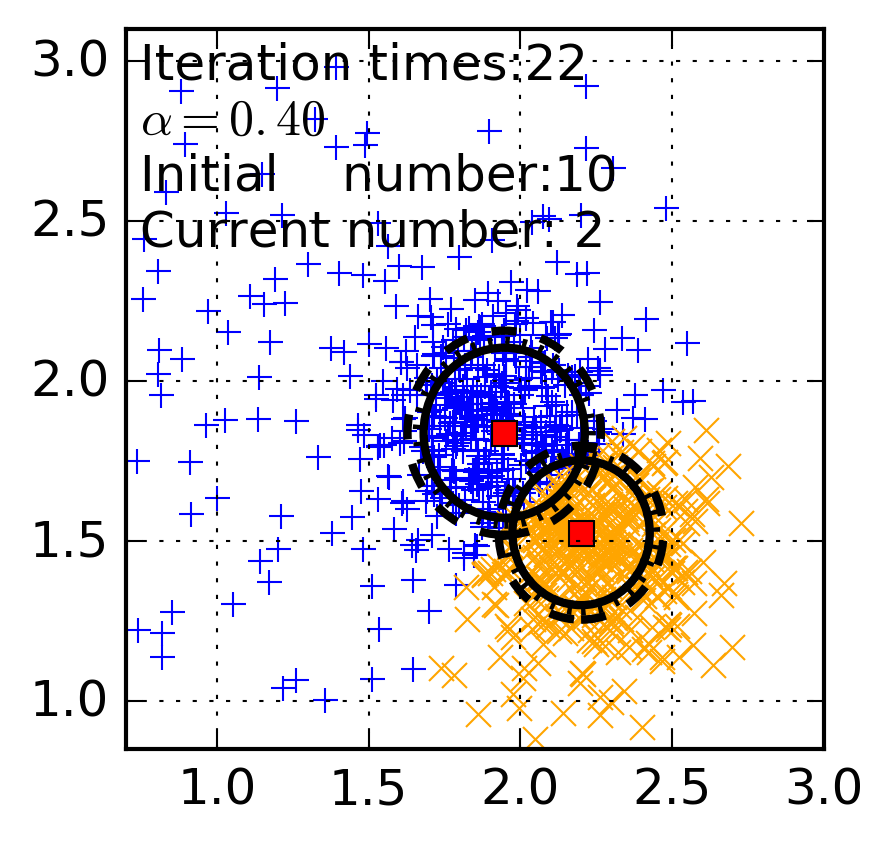
\includegraphics[width=0.33\textwidth]{img/example_close_cluster_last_frame_n_10_alpha_0_4.png}
  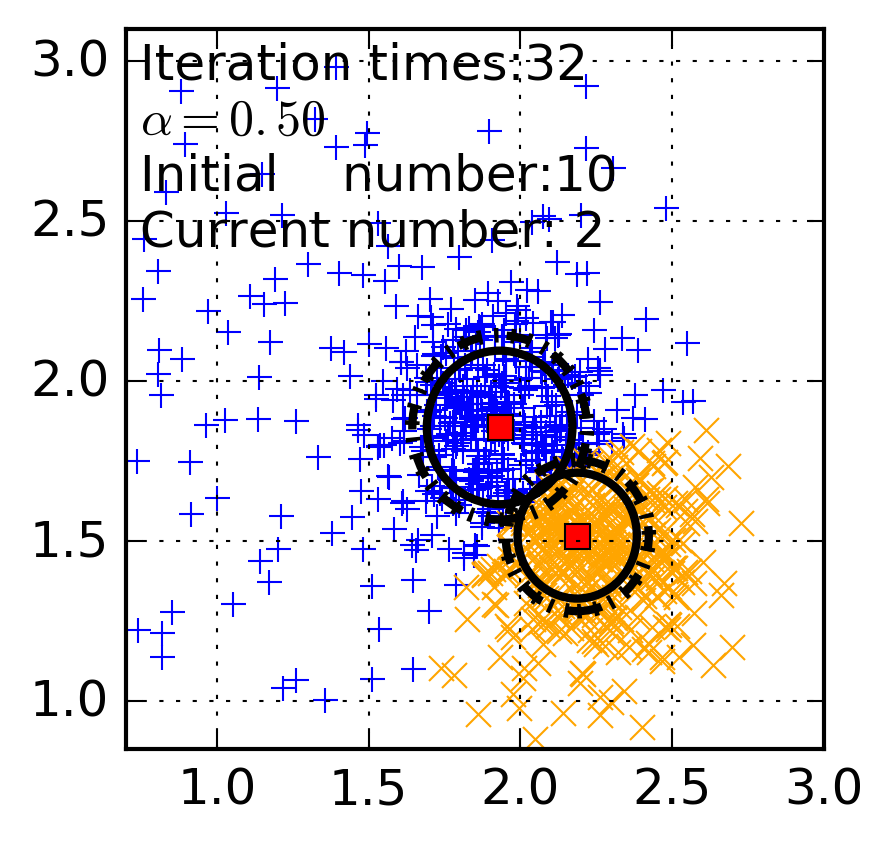
\includegraphics[width=0.33\textwidth]{img/example_close_cluster_last_frame_n_10_alpha_0_5.png}
  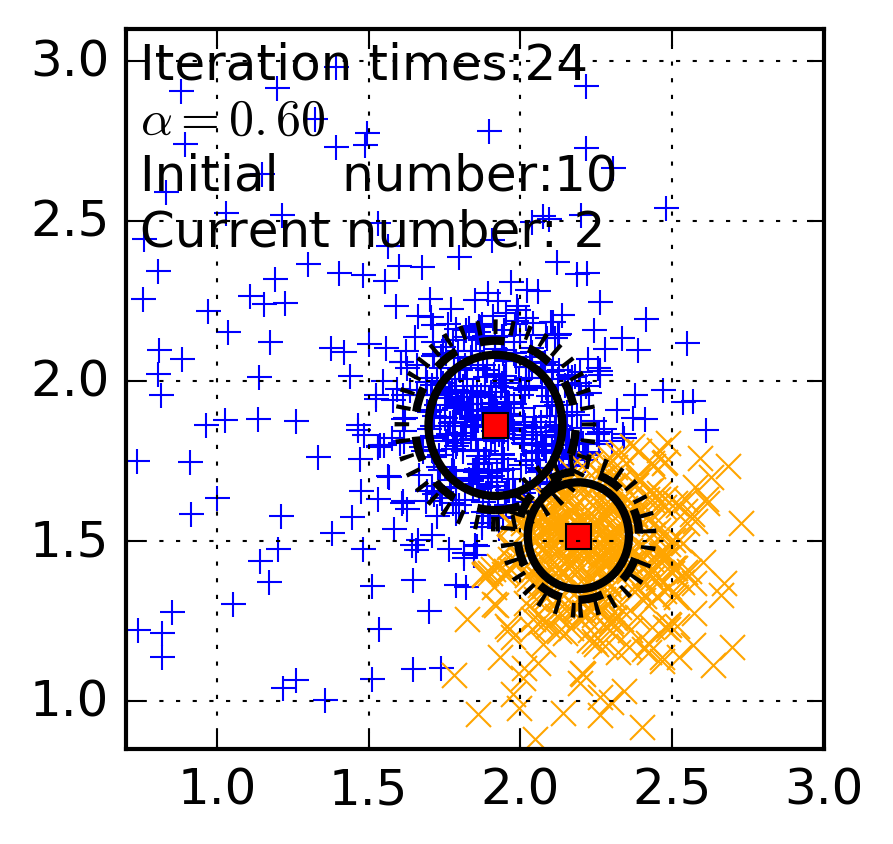
\includegraphics[width=0.33\textwidth]{img/example_close_cluster_last_frame_n_10_alpha_0_6.png}
\end{frame}

% Placing a * after \section means it will not show in the outline or
% table of contents.
\section*{Summary}

\begin{frame}{Summary}
  \begin{itemize}
  \item NPCM addresses the background noise cluster problem encountered in APCM and UPCM.
  \item NPCM exploits the intuition from UPCM to eliminate the parameter $\sigma_v$ basing on $\eta_j$.
  \item $\alpha$ is intuitive to choose and NPCM does not need strong prior information (e.g., the exact cluster number or the exact closeness of clusters) of the dataset.
  \end{itemize}
  
  \begin{itemize}
  \item Outlook
    \begin{itemize}
    \item Further researches can be conducted to reliably eliminate noise clusters in NPCM.
    \item Nonlinear shape clusters.
    \end{itemize}
  \end{itemize}
\end{frame}



% All of the following is optional and typically not needed.
\appendix
\section<presentation>*{\appendixname}
\subsection<presentation>*{For Further Reading}

\setbeamertemplate{bibliography item}{\insertbiblabel}
\begin{frame}[allowframebreaks]
  \frametitle<presentation>{References}
    
  \begin{thebibliography}{10}
    
 \setbeamertemplate{bibliography item}{\insertbiblabel}

  \bibitem{krishnapuram_possibilistic_1993}
R.~Krishnapuram and J.~M. Keller, ``A possibilistic approach to clustering,''
  \emph{IEEE Transactions on Fuzzy Systems}, vol.~1, no.~2, pp. 98--110, May
  1993.

\bibitem{nasraoui_improved_1996}
O.~Nasraoui and R.~Krishnapuram, ``An improved possibilistic {{C}}-{{Means}}
  algorithm with finite rejection and robust scale estimation,'' in \emph{Fuzzy
  {{Information Processing Society}}, 1996. {{NAFIPS}}., 1996 {{Biennial
  Conference}} of the {{North American}}}, Jun. 1996, pp. 395--399.

\bibitem{barni_comments_1996}
M.~Barni, V.~Cappellini, and A.~Mecocci, ``Comments on "{{A}} possibilistic
  approach to clustering",'' \emph{IEEE Transactions on Fuzzy Systems}, vol.~4,
  no.~3, pp. 393--396, Aug. 1996.

\bibitem{xenaki_novel_2016}
S.~D. Xenaki, K.~D. Koutroumbas, and A.~A. Rontogiannis, ``A {{Novel Adaptive
  Possibilistic Clustering Algorithm}},'' \emph{IEEE Transactions on Fuzzy
  Systems}, vol.~24, no.~4, pp. 791--810, Aug. 2016.

\bibitem{hou_pcm_2016}
P.~Hou, H.~Deng, J.~Yue, and S.~Liu, ``{{PCM}} and {{APCM Revisited}}: {{An
  Uncertainty Perspective}},'' \emph{arXiv:1610.08624 [cs, stat]}, Oct. 2016.

\bibitem{wang_new_2016}
L.~X. Wang, ``A {{New Look}} at {{Type}}-2 {{Fuzzy Sets}} and {{Type}}-2
  {{Fuzzy Logic Systems}},'' \emph{IEEE Transactions on Fuzzy Systems},
  vol.~PP, no.~99, pp. 1--1, 2016.

  \end{thebibliography}
\end{frame}
\end{document}



%%% Local Variables:
%%% mode: latex
%%% TeX-master: t
%%% End:
